
The previous chapter introduced QRNNs and DRNNs as machine-learning based
methods to perform remote sensing retrievals. The motivation for this was to
find a practical approach to combine the expressiveness of modern, deep neural
networks with the theoretically sound handling of uncertainties of conventional
inverse-theory-based retrieval methods. To explore the validity and
practicality of the proposed methods we have tested them using idealized
scenarios and developed multiple real-world retrieval applications. This section
presents this work and summarizes the main results.

\section{Handling retrieval uncertainty with neural networks}

The first of the append papers, titled \textit{A neural network approach to
estimating a posteriori distributions of Bayesian retrieval problems} and
published in \citet{pfreundschuh18},} proposes the use of QRNNs for remote
sensing retrievals. The motivation for this study were the shortcomings the
retrieval methods that were available at the time of its writing. The Bayesian
framework provides a principled way of handling the retrieval uncertainties
(see Sec.~\ref{sec:machine_learning:retrieval_problem}), but the commonly used
methods are computationally complex. While retrievals based on neural networks
were already common and often offered superior performance  in terms of
computational cost as well as accuracy, they typically neglected retrieval
uncertainties.

The aims of the study were two-fold: (1) To demonstrate the compatibility of
QRNNs with conventional Bayesian retrieval methods and (2) to demonstrate the
practicality of QRNNs by applying them to a real-world retrieval application.

To demonstrate the compatibility of QRNNs with conventional Bayesian retrieval
methods, we made use of an idealized but realistic retrieval scenario, in which
the true Bayesian solution could be calculated to arbitrary precision. We then
used QRNNs and Bayesian Monte Carlo Integration (BMCI), a commonly used Bayesian
retrieval method, to solve the retrieval and compared the solutions to the true
solution. BMCI calculates an approximate solution of the retrieval problem using
a database of observations and corresponding reference values. This makes it
similar in this regard to a machine learning method. We found that QRNNs work at
least as good as BMCI in solving the retrieval problem when both are based on a
sufficiently large dataset. For smaller datasets, there was a clearer advantage
for QRNNs indicating that they cope better with the curse of dimensionality.

This first result has two important implications. Firstly, it showed that QRNNs
can be used instead of BMCI and expected to work at least as good given the same
training data. Even if the advantage of neural networks over BMCI on the
considered dataset was marginal when sufficient training data is available, the
use of neural networks offers distinct advantages. For one, the time required to
produce a neural network prediction is independent of the training data size.
This is not the case for BMCI, for which this time scales linearly with the size
of the training database. This means that the amount data that can be used by
the method may be limited by operational processing requirements. Besides that,
because of the flexibility of QRNNs they can be easily extended to image or time
series data, which is again not the case for BMCI. The second important
implication of these results was that it showed the compatibility of
probabilistic machine learning methods with the Bayesian retrieval methods.
These results link the extensive theory on Bayesian retrieval methods
\citep{rodgers00, tarantola05} with and machine-learning-based retrieval
methods. The correspondence between the training data of the neural network and
the a priori distribution of a Bayesian retrieval, highlights the role the a
priori distribution plays for the retrieval results and accurate quantification
of retrieval uncertainties.


%Two experiments were performed in the study. The first one used an idealized
%retrieval scenario in which samples from the posterior distribution $p(y|x)$
%could be calculated using Markov Chain Monte Carlo (MCMC) methods. MCMC is
%generally too slow to be used in operational processing, but its ability to
%generate samples from the true posterior distribution makes it suitable to
%provide a reference solution against which QRNNs and another Bayesian retrieval
%method could be evaluated. A principal results from this experiment is shown
%Fig.~\ref{fig:contributions:cdfs_qrnn_bmci}. The plot displays the retrieved
%CDFs of the posterior distributions using QRNN and Bayesian Monte Carlo
%Integration (BMCI), which is a commonly used Bayesian retrieval methods. Each
%panel shows the reference CDF obtained using MCMC in the background and the CDFs
%obtained using BMCI in blue, those obtained from a single QRNN using a solid red
%line and those obtained from an ensemble of QRNNs using red markers. The shown
%samples were chosen according to the Kolmogorov-Smirnov of the BMCI
%($\text{KS}_\text{BMCI}$) and QRNN ($\text{KS}_\text{QRNN}$), which measures
%the agreement between the reference and retrieved CDF, and thus show retrieval
%results of varying quality from each retrieval.
%
%The main finding from this first experiment is that the CDFs retrieved using
%QRNN and BMCI agree very well with the reference CDF calculated using MCMC. This
%indicates that probabilistic neural network retrievals are consistent with the
%Bayesian solution of inverse problems with the a priori distribution being
%represented by the training data.
%
%\begin{figure}
%  \centering
%  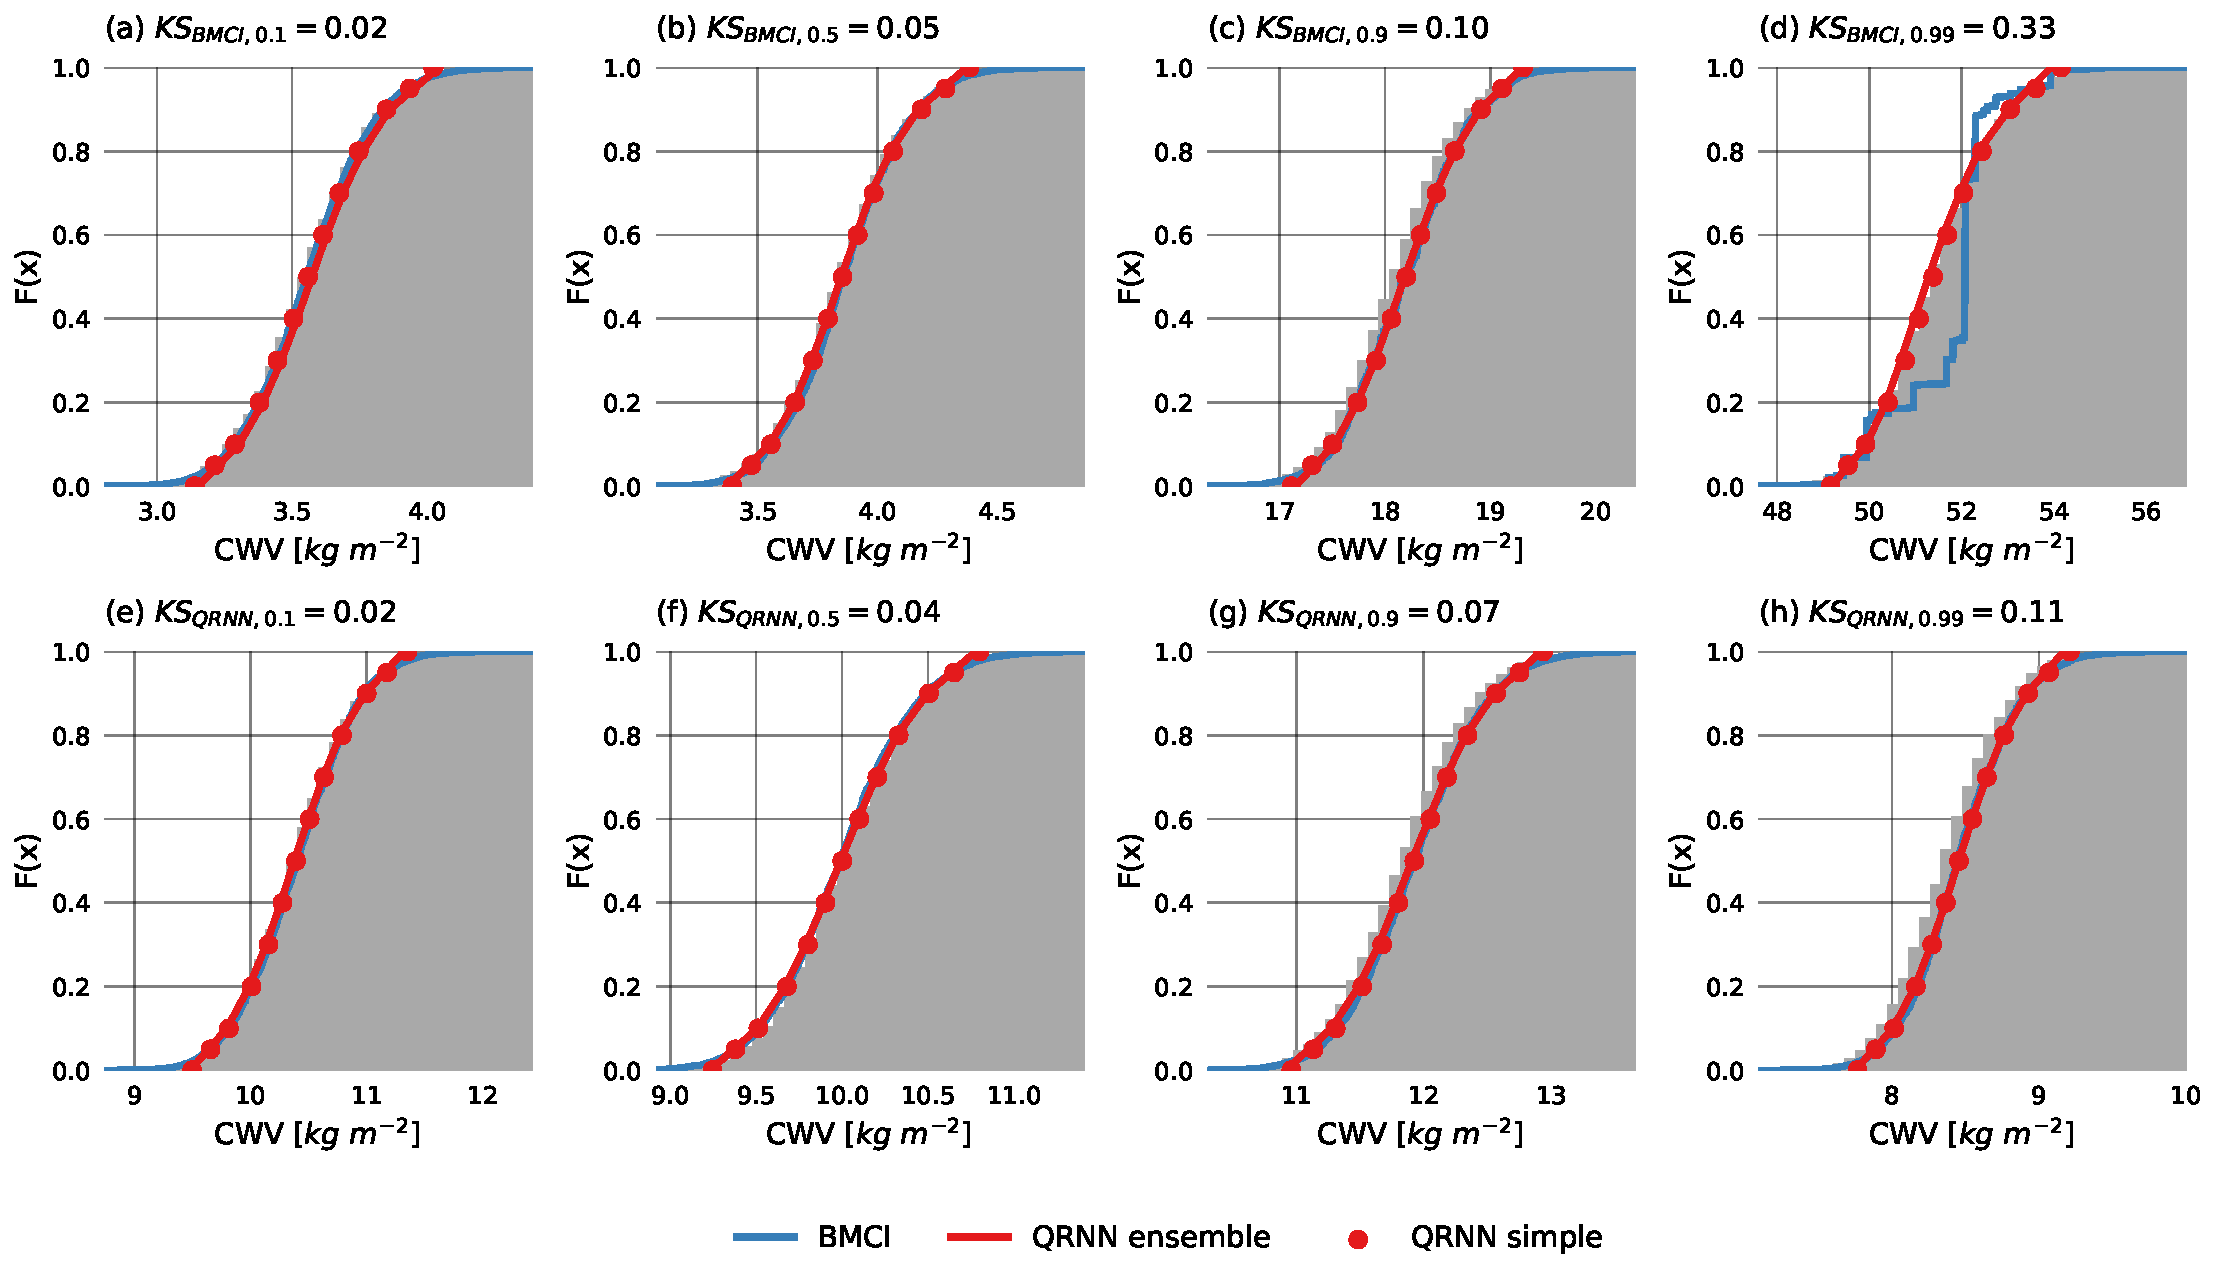
\includegraphics[width=\textwidth]{cdfs_qrnn_bmci}
%  \caption{ Retrieved a posteriori CDFs obtained using MCMC (gray), BMCI (blue),
%    a single QRNN (red line) and an ensemble of QRNNs (red marker). Cases
%    displayed in the first row correspond to the 1st, 50th, 90th and 99th
%    percentiles of the distribution of the Kolmogorov– Smirnov statistic of BMCI
%    compared to the MCMC reference. The second row displays the same percentiles
%    of the distribution of the Kolmogorov–Smirnov statistic of the single-QRNN
%    predictions compared to MCMC.}
%  \label{fig:contributions:cdfs_qrnn_bmci}
%\end{figure}

The second experiment from this study applied QRNNs to the retrieval of cloud
top pressure (CTP) from infrared observations from the Moderate Resolution
Imaging Spectroradiometer (MODIS). Comparison of the QRNN retrieval to an
existing retrieval using a deterministic neural network showed that QRNNs yield
comparable or better accuracy for point predictions with the added benefit of
providing reliable uncertainty estimates. In particular, we show the ability of
the QRNN to represent non-Gaussian retrieval errors and the superiority over
commonly assumed Gaussian error models. A consequence of these findings was the
adoption of QRNNs for the operational production of near real-time retrievals of
cloud top pressure at the European Organisation for the Exploitation of
Meteorological Satellites.

\section{Passive microwave precipitation retrievals}

The second study included in thesis, titled \texti{%
GPROF-NN: A neural network based implementation of the Goddard Profiling Algorithm %
} and published as \citet{pfreundschuh22a}, applied the QRNN methodology to
the retrieval of precipitation from PMW observations of the GPM mission.
GPM  is an international satellite mission lead by NASA and JAXA, which aims
to provide global measurements of precipitation at high spatial and temporal
resolution. The mission is built around the Core Observatory satellite, which
carries a precipitation radar and a PMW sensor dedicated to
the remote sensing of precipitation. Retrievals from the combined radar/PMW
observations from the Core Observatory are used to build a retrieval
database that is in turn used to for the retrievals of a constellation 
PMW sensors. As of this writing, the GPM constellation comprises 9 active
satellites.

The algorithm that is used to retrieve precipitation from GMI, the PMW sensor on
the Core Obsevatory, and the other PMW sensors of the GPM constellation is the
Goddard Profiling Algorithm (GPROF, \citeauthor{kummerow15},
\citeyear{kummerow15}). GPROF is based on the BMCI method and retrieves surface
precipitation as well as profiles of hydrometeor concentrations and latent
heating rates. The aim of the study was to assess the potential benefits of
replacing BMCI with a neural network based retrieval. Besides that, the study
aimed to explore to what extent the accuracy of the retrieval can be improved if
structural information from neighboring pixels is incorporated into the
retrieval instead of processing each pixel separately as the current
implementation does. To this end, two neural network based implementation were
developed. The first one, named GPROF-NN 1D, uses an MLP to retrieve
precipitation from a single pixel. The second one, GPROF-NN 3D, uses a CNN to
retrieve precipitation across the full swath simultaneously. This allows the
retrieval to leverage structural information in the observations, which is not
available to the two other implementations.

Both the GPROF-NN 1D and GPROF-NN 3D retrieval were developed to be functionally
equivalent to the currently operational GPROF algorithm so that they can
potentially replace it in an upcoming update. Moreover, the implementations were
restricted to use exactly the same data for their training as the current method
to ensure that the comparison of the three methods only reveals differences
between the retrieval methods. This required the development of a training
pipeline that can be applied to all sensors of the GPM constellation.

While the application of QRNNs to the GPROF algorithm is straight-forward from a
theoretical perspective, the requirements of developing a retrieval that uses
identical input data, produces equivalent outputs and uses the same data as the
current implementation of GPROF proved challenging. The training data for the
sensors of the GPM constellation makes use of radiative transfer simulation,
however these are generated not for full satellite swaths of observations but
only for single pixels this made the raw training data unsuitable for the
training of a CNN. Since extending the simulations to the full swath is
currently not possible, we trained an intermediate CNN-based 'retrieval' to
emulate the simulation of PMW observations.

%proved challenging especially for the GPROF-NN 3D retrieval. The training data
%for all sensors of the GPM constellation is based on combined radar/radiometer
%observations from the GPM satellite. Since these observations are only available
%at a $\SI{100}{\kilo \meter}$-wide swath at the center of the GMI observations,
%a way had to be found to extent these to the full GMI-swath and to remap them to
%the viewing geometries of the other sensors. The current approach uses an
%intermediate simulator network to extend the simulated observations to the full
%swath of GMI, which are then remapped to the viewing geometries of other sensors
%by interpolation. This solution should be a considered a heuristic that was
%pursued mainly because extending the simulations that are routinely performed
%for the generation of the GPROF training data would have been outside the scope
%of this study.

The main results from this study are estimates of potential improvements in
retrieval accuracy that can be realized by upgrading GPROF to either the
GPROF-NN 1D or GPROF-NN 3D retrieval. We found consistent improvements for the
GPROF-NN 1D algorithms across a range of accuracy metrics and across all
retrieved quantities. The accuracy is improved further by the GPROF-NN 3D
retrieval, which yields improvements similar in magnitude to those provided by
the GPROF-NN 1D algorithm of the GPROF baseline retrieval. Furthremore, we found
that the effective resolution of the retrieval improves by at least
$\SI{40}{\percent}$ with the neural network based retrieval. The study included
results from two case studies of Hurricane overpasses from the GMI and MHS
sensors, which provided limited evidence that the retrieval improvements can be
expected to carry over to real observations.

Although the results from this study were promising, their significance was
limited because the evaluation of the retrieval was limited to the same source
of data, which was used for the generation of the training data. Since the
objective of the study was to compare the BMCI retrieval method and QRNNs, this
simplification was justified because in an validation against independent data,
the benefits of the neural-network-based retrieval may have been masked by
deviations of the training data from the validation data. However, the
practically more relevant question was to what extent do these improvements
carry over to comparison against independent validation data.

We aim to address this question in a study that is currently under preparation
and included in this thesis as the third paper, titled \texit{% Evolution of the
GPROF passive microwave precipitation retrievals evaluated against ground
radar measurements over the continental US and the Pacific Ocean% }. Since the
development of the GPROF-NN algorithms was performed in parallel with a new
version of the GPROF retrieval, this study aimed to assess improvements in
this new version of GPROF (GPROF V7) against the previous version (GPROF V5)
and assess the potential benefits of replacing GPROF with GPROF-NN 1D or 3D in
a future update. Furthermore, the study aims to identify  potential outstanding issues
impeding the adaptation of the GPROF-NN retrievals to operational processing.

The validation is based on ground-radar measurements of precipitation
specifically created for the validation of GPM measurements. It is
based measurements from the continental United States (CONUS) and a ground radar
station on the Kwajalein atoll in the Pacific Ocean to complement the primarily
land-based observations over CONUS with observations over ocean.

The main focus of this study are retrievals from the GMI radiometer, which plays
a special role in the GPM constellation due to it placement on the Core
Observatory together with the precipiation radar and it being designed
specifically for the retrieval of precipitation. The accuracy of the
precipitation retrieved from the GMI sensor using the two version of the
conventional GPROF algorithm as well as the two GPROF-NN is evaluated for two
years of co-locations. The results clearly show that the benefits of the
neural-network-based implementation of GPROF carry over to validation against
independent precipitation measurements. In particular, we find that the
effective resolution of the retrieved precipitation improves by more than
a factor of 2 over land.

In addition to GMI, we also investigated the retrieval accuracy other sensors of
the GPM constallation using one year of observations over the CONUS as the
training for these sensors is completed. For the two sensors that we have
assessed we also find improvements in retrieval accuracy. This is an encouraging
result because the training for them is derived from simulated observations,
while it is derived from real observations for GMI.


\section{VIS/IR precipitation retrievals}

While the neural-network-based implementation of GPROF provided clear evidence
for the potential of neural-network based precipitation retrievals, the
constraint of a retrieval that provides the same output as the currently
operational GPROF algorithm limited the exploration of retrieval improvements to
currently available retrieval outputs. The assessments presented in
\citet{pfreundschuh22} and \citet{pfreundschuh22c} therefore focused mostly on
deterministic precipitation estimates and thus did not explore the full
potential of the probabilistic predictions afforded by the neural network.

The aim of the study presented in \citet{pfreundschuh22b} was to explore the
full potential of probabilistic neural-network based precipitation retrievals in
the context of near real-time retrievals from VIS/IR observations over Brazil.
The input data for the retrieval comes from the advanced baseline imager (ABI)
on the geostationary operational environmental satellite (GOES) 16. To train the
retrieval, the input observation were co-located with combined radar-radiometer
measurements from the GPM core observatory satellite.

To validate the retrieval its results were compared to 1 month of gauge
measurements. The retrieval accuracy was assessed by comparing it to the
retrieval algorithm that is currently used operationally at the Brazilian
institute of space research as well as to commonly used global precipitation
retrievals. We were able to show that, despite the limited information content
of VIS/IR observations, deep-learning-based retrievals outperform currently
available methods, even those that merge IR observations from geostationary
satellite with PMW observations polar-orbiting platforms.

Furthermore, the study explored the potential of the probabilistic precipitation
estimates. We were able to show that, after correcting for differences in the
precipitation statistics of the training data and gauge measurements, confidence
intervals derived from the probabilistic predictions were well calibrated
against the gauge measurements. We also provided results that the probabilistic
predictions improve the detection of heavy precipitation.


\section{Cloud correction for data assimilation}

The final study included in this thesis explores the application of QRNNs to
remove the effect of clouds from microwave observations. The observations
contain important information on the distribution water vapor in the atmosphere
and are used in data assimilation systems to find good initial conditions for
numerical weather forecasts. However, the presence of hydrometeors in the
atmosphere makes radiative transfer calculation much more complex which
complicates the use of observations. Since the information on the hydrometeors
themselves is not really used in the data assimilation system, a model that
could accurately predict how these observations would look when the effect of
the hydrometeors was removed, would allow these observations to in a less
complex and computationally more efficient way.

Because of their impact on the radiative transfer, operational data assimilation
systems have to detect observations that are affected by clouds to either
correctly handle them if the DA system is sufficiently advanced to handle cloudy
observations or to discard them altogether. The first experiment therefore
assessed the potential of applying QRNN to correct cloud-contaminated
observations from an existing sensor and compared the performance to existing
methods. The experiment showed that the QRNN-derived correction leads to a lower
bias in the observations than the residual biases in currently used filtering
methods, which reject up to $\SI{30}{\percent}$. The important point here is that the QRNN-based
cloud correction achieves this without rejecting any observations, which would
makes more observations available to the data assimilation system.

The second experiment then extended the approach to a soon-to-be-launched and
and a hypothetical satellite sensor. Both of the will carry microwave sensors
with channels above $\SI{300}{\giga \hertz}$. These high frequencies make the
observations more sensible to scattering from ice particles, which further
complicates their use in data assimilation. In these cases QRNN-based cloud
correction would provide a simple alternative to ingesting this information into
data assimilation systems by using the hydrometeor information afforded by the
high-frequency channels to improve the removal of cloud contamination at lower
frequency channels. The results show that channels at frequencies exceeding
$\SI{300}{\giga \hertz}$ are well suited for cloud correction.

This study proposed a novel application of QRNNs for the correction of microwave
observations for use in data assimilation and retrievals of water vapor
profiles. QRNN-based cloud correction provides superior performance to existing
methods. In addition to that, the predicted uncertainties provide more accurate
error estimates than currently used error models for data assimilation.
Finally, the simulation-based assessment of the potential of microwave observations
at sub-millimeter wavelength lead to the selection of these channels for an
upcoming satellite mission \citep{arctic_weather_satellite}.

\section{Future work}

The findings of this thesis suggests several directions of future research.
These will be discussed below.

\subsection{Handling retrieval uncertainty with neural networks}

This thesis has proposed and assessed to neural-network-based methods for
handling uncertainties in remote sensing retrievals and shown their practicality
across multiple retrieval applications. The advantage of these methods is
certainly their simplicity. Only a minor modification in the training process is
required to migrate a deterministic neural network retrieval to a probabilistic
one.

There are, however, two important limitations of the approaches: Their
incapability of handling correlations in the retrieval outputs and their
reliance on the aleatoric assumption, which postulates that the predictive
uncertainty is dominated by the aleatoric uncertainty.

It would therefore be valuable to systematically evaluate the approaches against
Bayesian neural networks and generative model on a set of atmospheric retrieval
problems. In particular, it would be important to evaluate the methods not only
with respect to retrieval accuracy but to also take into account the effect on
downstream applications of the data. This would provide guidance in what scenarios
the computationally more complex alternative approaches should be applied.

\subsection{GPM precipitation retrievals}

Due to the good performance of the developed GPROF-NN retrievals, they are being
considered for operational implementation for the PMW precipitation retrieval of
the GPM mission. This will require some additional investigations regarding the
climatological stability of the GPROF-NN retrievals across different satellites.

In addition to that, the migration to a neural-network-based implementation
opens up for a number of improvements of the GPROF retrieval. One of them is the
extension of the training data to cover multiple years of observations. As was
found in \citep{pfreundschuh22c}, this may improve the climatic stability of the
retrieval. Furthermore, including samples from the posterior distribution may
improve the representation of extreme precipitation in the retrieval results,
which is relevant for climatological studies.

\subsection{VIS/IR precipitation retrievals}

The results presented in \citet{pfreundschuh22b} clearly showed the
potential of deep neural networks for precipitation retrieval from
geostationary satellites. According to personal communication, the
developed retrieval is also considered for operational application.

An interesting result that emerged from this study was that, despite the low
information content of the geostationary observations on precipitation,
deep-learning-based retrievals can outperform highly complex retrieval pipelines
which integrate observations from multiple sensors. This indicates that the use
of information in multi-sensor retrievals is sub-optimal. In a future project,
we will therefore explore the potential of fusing observations from different
sensors directly using a single neural network.
